\documentclass[11pt]{article}
\usepackage[margin=1in]{geometry}
\usepackage{graphicx}
\usepackage{amsmath}
\usepackage{booktabs}
\usepackage{siunitx}
\usepackage{hyperref}
\usepackage{caption}
\usepackage{subcaption}
\usepackage{float}

\title{Vehicle Dynamics Simulation Model Overview}
\author{Vehicle-Dynamics-Sim-Can}
\date{\today}

\begin{document}
\maketitle

\begin{abstract}
This document provides a readable, end-to-end overview of the vehicle dynamics model implemented in the simulator. It is written for a general engineering audience and for readers who are new to vehicle dynamics simulation. The focus is on explaining model structure, the key physical assumptions, and the major tunable parameters. We also document the low-speed behavior fixes (kinematic blending and tire relaxation) and show representative simulation plots.
\end{abstract}

\tableofcontents
\newpage

\section{Purpose and Scope}
The simulator implements a lightweight vehicle dynamics model intended for closed-loop control testing and fast iteration. It is not a full-fidelity multi-body model; instead it uses a reduced-order 3-DOF rigid body model with simplified powertrain and tire behavior. This model is designed to be:

\begin{itemize}
\item Fast enough for real-time closed-loop simulation.
\item Understandable and tunable through a YAML vehicle configuration.
\item Stable for common test maneuvers and controller development.
\end{itemize}

\section{System Architecture}
The simulator is built as three primary subsystems that execute in a fixed order each timestep:

\begin{enumerate}
\item \textbf{SteerSubsystem}: Converts steer command into front-wheel angles using Ackermann geometry and rate limits.
\item \textbf{DriveSubsystem}: Converts torque/brake commands into longitudinal forces and lateral tire forces.
\item \textbf{VehicleSubsystem}: Integrates the vehicle body states (position, velocity, yaw) using forces from the drive subsystem.
\end{enumerate}

Each subsystem updates a shared \texttt{PlantState}. The closed-loop controller sends commands over a virtual CAN bus and receives state feedback frames.

\section{State and Coordinate Definitions}
The vehicle model uses a body-fixed coordinate frame:

\begin{itemize}
\item $x$ axis forward, $y$ axis left, yaw positive counter-clockwise.
\item Longitudinal velocity $v$ (\texttt{v\_mps}) and lateral velocity $v_y$ (\texttt{vy\_mps}) are expressed in the body frame.
\item Yaw rate $\dot{\psi}$ (\texttt{yaw\_rate\_radps}) is around the vertical axis.
\end{itemize}

The global position $(x, y)$ is obtained by rotating body velocities into the world frame each timestep.

\section{Steering Model}
The steering model uses:

\begin{itemize}
\item Ackermann geometry for inner/outer wheel angles.
\item A steer angle rate limit (hydraulic steering response).
\item Speed-based steering reduction.
\item An additional low-speed steering clamp to prevent yaw oscillations.
\end{itemize}

The steering clamp is a simple linear ramp: the maximum steer angle is reduced at very low speeds and reaches full authority above a specified speed.

\section{Powertrain and Longitudinal Forces}
Longitudinal forces are computed from torque and brake commands:

\begin{itemize}
\item Motor torque is limited by maximum torque, power, drivetrain efficiency, and surface friction.
\item Brake force is based on a maximum brake torque and a front/rear bias.
\item Static rolling resistance and quadratic aerodynamic drag are applied.
\end{itemize}

These forces generate longitudinal acceleration, and the vehicle velocity is clamped to forward and reverse limits.

\section{Tire and Lateral Force Model}
Lateral forces use a linear tire model:

\begin{equation}
F_y = -C_y \alpha
\end{equation}

where $C_y$ is the cornering stiffness and $\alpha$ is the slip angle. To avoid instability near standstill, slip angles are scaled to zero as speed goes to zero, and a friction circle saturation clamps lateral forces.

\subsection{Tire Relaxation (First-Order Lag)}
To reduce high-frequency oscillations, lateral forces are passed through a first-order lag:

\begin{equation}
F_{y}(t+\Delta t) = F_y(t) + \alpha (F_{y,\text{target}} - F_y(t))
\end{equation}

where

\begin{equation}
\alpha = \frac{\Delta t}{\tau + \Delta t}
\end{equation}

and $\tau$ is the tire relaxation time constant (configurable in YAML).

\section{Vehicle Body Dynamics (3-DOF)}
The vehicle body integrates longitudinal, lateral, and yaw dynamics. In body coordinates, the longitudinal acceleration is:

\begin{equation}
\dot{v}_x = \frac{F_x}{m} + v_y \dot{\psi}
\end{equation}

The coupling term $v_y\dot{\psi}$ can dominate at low speed. This is why low-speed stabilization is essential.

\section{Low-Speed Stabilization}
Two key stabilizers are used:

\subsection{Kinematic Blend}
Below a configurable speed $v_{\text{blend}}$, yaw rate and lateral velocity are blended toward a kinematic bicycle model:

\begin{equation}
\dot{\psi}_{\text{kin}} = \frac{v}{L} \tan(\delta)
\end{equation}

This prevents unrealistic oscillations when the vehicle is nearly stationary.

\subsection{Yaw Damping}
An additional low-speed yaw damping term is applied to reduce oscillations. This is a simple linear damping proportional to yaw rate.

\section{Configuration and Tuning}
Vehicle parameters are loaded from YAML files. Key tunables include:

\begin{itemize}
\item Mass, wheelbase, track width, CoG position, yaw inertia.
\item Motor torque/power limits and brake torque.
\item Rolling resistance and drag.
\item Cornering stiffness values.
\item \textbf{Low-speed kinematic blend threshold} \texttt{v\_kinematic\_blend\_mps}.
\item \textbf{Tire relaxation time constant} \texttt{tire\_relax\_tau\_s}.
\end{itemize}

\section{Simulation Example}
Figure~\ref{fig:results} shows a typical closed-loop run. The plots illustrate:

\begin{itemize}
\item Vehicle trajectory.
\item Speed, longitudinal acceleration, and coupling term.
\item Steering commands and yaw response.
\item Motor torque and brake force.
\item Wheel speeds.
\item Lateral velocity and yaw rate.
\end{itemize}

\begin{figure}[H]
    \centering
    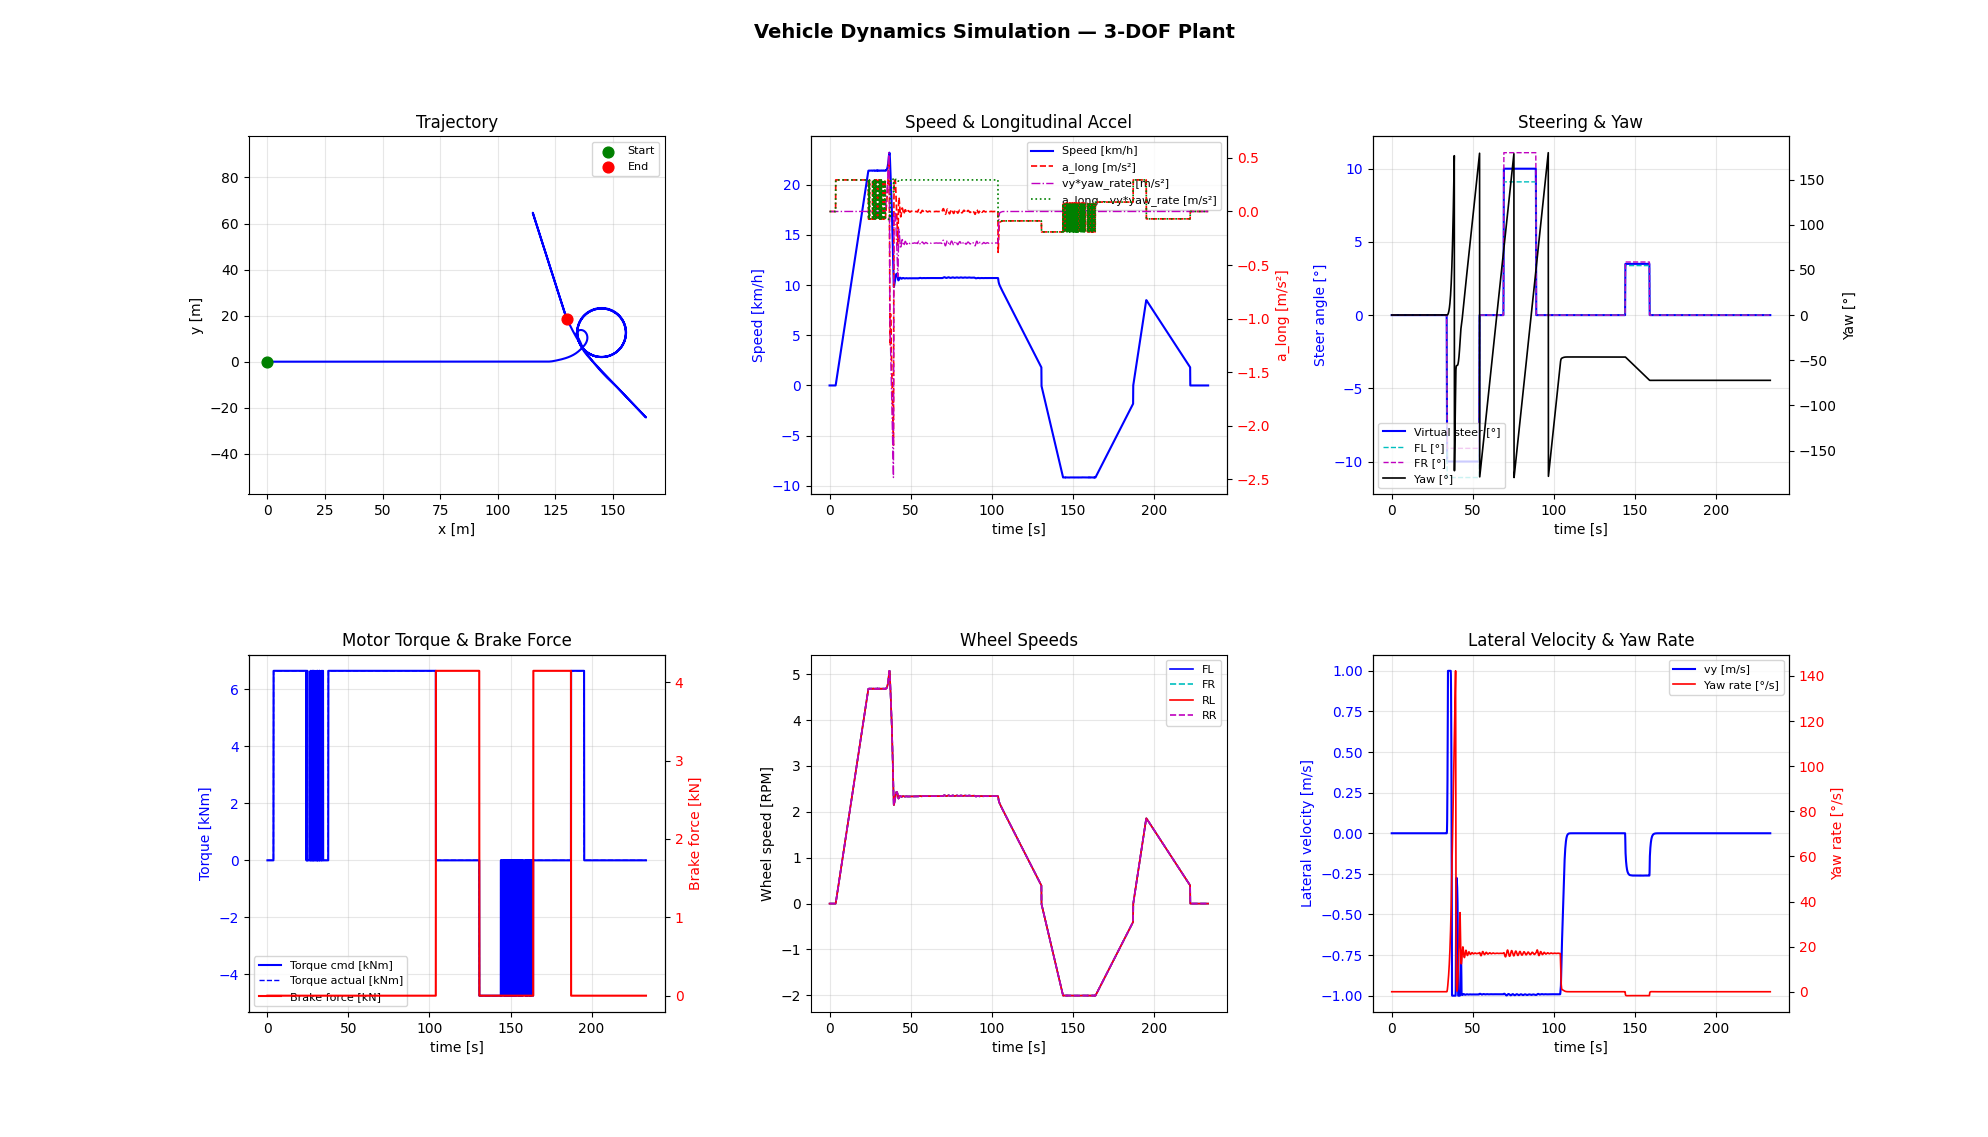
\includegraphics[width=0.95\textwidth]{../Results.png}
    \caption{Closed-loop simulation results from \texttt{sim\_out.csv}.}
    \label{fig:results}
\end{figure}

\section{Tuning Guide (Quick Reference)}
This section provides a short, practical tuning guide for common issues. Use it as a quick checklist before changing the controller.

\begin{itemize}
\item \textbf{Yaw oscillation at low speed}: increase \texttt{v\_kinematic\_blend\_mps} or increase yaw damping.
\item \textbf{Overly wide reverse turn}: increase \texttt{REV\_STEER\_DEG} or \texttt{Cy\_rear\_Npm}.
\item \textbf{Harsh speed transitions}: increase tire relaxation time constant \texttt{tire\_relax\_tau\_s}.
\item \textbf{Excessive lateral drift}: lower \texttt{v\_lat\_max\_mps} or reduce steer command.
\end{itemize}

\begin{table}[H]
\centering
\caption{Key tuning parameters and suggested ranges}
\begin{tabular}{@{}llp{3.5in}@{}}
\toprule
\textbf{Parameter} & \textbf{Typical Range} & \textbf{Effect} \\
\midrule
\texttt{v\_kinematic\_blend\_mps} & 1.5--3.5 & Low-speed stability and smooth turning. \\
\texttt{tire\_relax\_tau\_s} & 0.2--0.5 & Reduces high-frequency oscillations. \\
\texttt{Cy\_front\_Npm} & 2.0--3.0e6 & Front lateral response / turn-in. \\
\texttt{Cy\_rear\_Npm} & 2.0--3.2e6 & Rear stability / understeer balance. \\
\texttt{yaw\_inertia\_kgm2} & 6--9e6 & Overall yaw responsiveness. \\
\texttt{REV\_STEER\_DEG} & 15--25 & Reverse turn tightness. \\
\bottomrule
\end{tabular}
\end{table}

\section{Glossary (Short)}
\begin{itemize}
\item \textbf{Yaw}: Vehicle heading angle in the horizontal plane.
\item \textbf{Yaw rate}: Rate of change of yaw (turning speed).
\item \textbf{Slip angle}: Angle between wheel pointing direction and actual velocity.
\item \textbf{Cornering stiffness}: Slope of lateral force vs. slip angle.
\item \textbf{Kinematic bicycle}: A geometry-based turning model used at low speed.
\end{itemize}

\section{Limitations and Future Work}
This model is intentionally simplified. The main limitations are:

\begin{itemize}
\item Linear tire model (no combined-slip dynamics beyond friction circle clamp).
\item No full wheel rotational dynamics or drivetrain inertia.
\item No suspension or load transfer modeling.
\item Simplified steering and brake models.
\end{itemize}

Potential future improvements include: richer tire models, more realistic steering compliance, and a flexible switch between kinematic and dynamic modes.

\section{Summary}
The simulator provides a practical balance between realism and simplicity. With the low-speed stabilizers, it produces stable closed-loop behavior suitable for controller development. The YAML configuration exposes the key knobs for tuning, while keeping the model approachable to non-specialists.

\end{document}
